%!TEX root = ../thesis.tex
%*******************************************************************************
%****************************** Chapter 3 appendix *********************************
%*******************************************************************************
\chapter{Appendix to Chapter 5}\label{appx:siren}

\graphicspath{{04_SIREN/Figs/}}

% \section{Sequencing}\label{appendix:sequencing}

% \begin{figure}[htbp!]
%     \centering
%     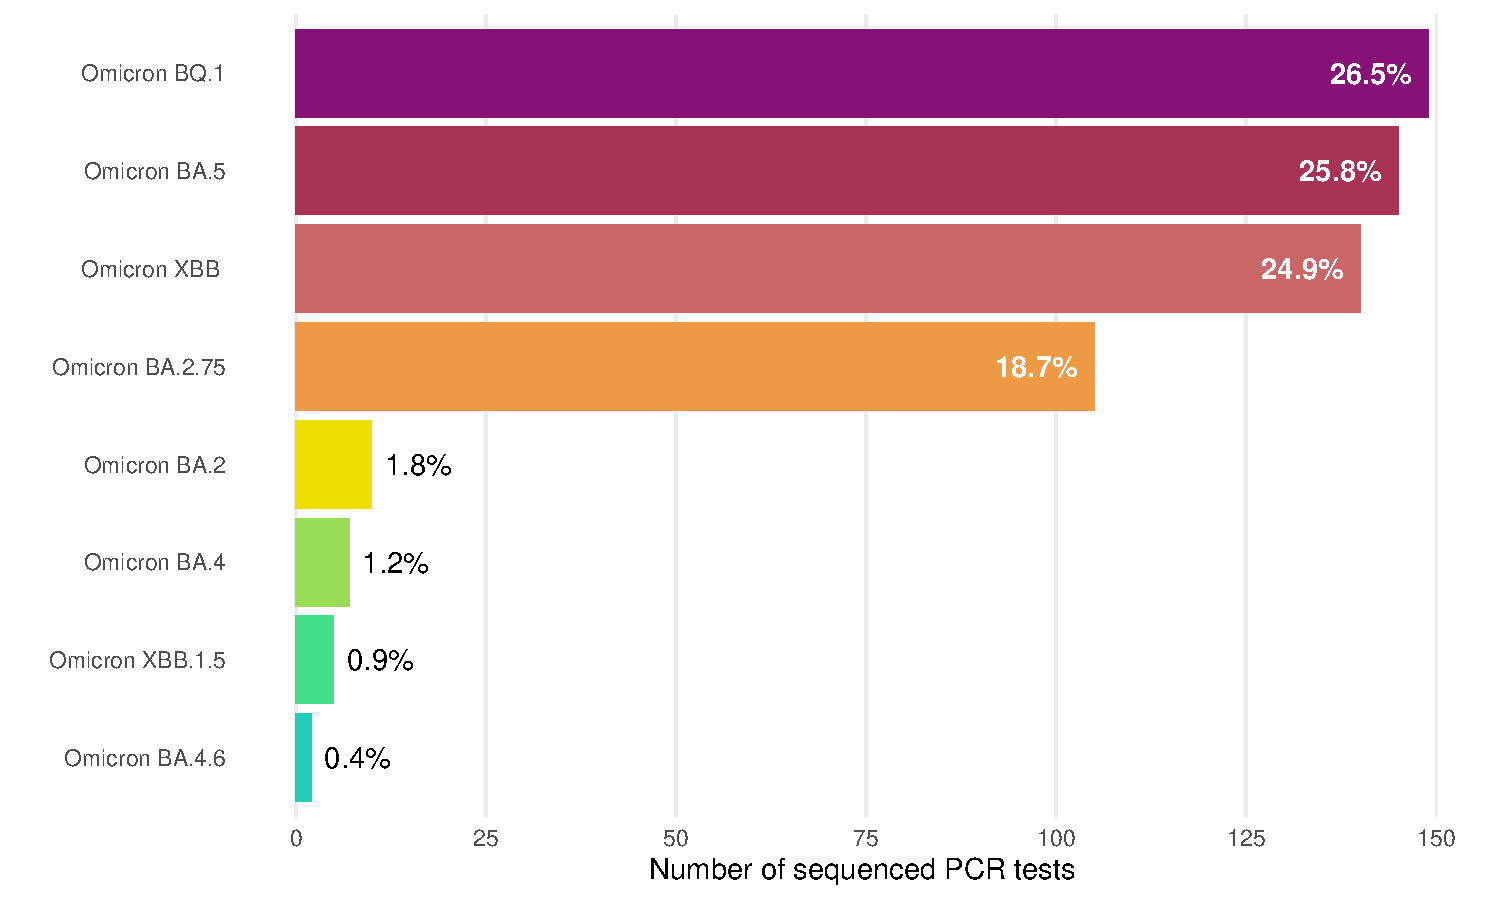
\includegraphics[width=\textwidth]{interim4_sequences.pdf}
%     \caption{SARS-CoV-2 infections, by sequenced variant. Percentages indicate proportion of sequenced variants. Sequence information was available for 43.4\% (563/1,298) of detected infections.}\label{fig:sequences}
% \end{figure}

\begingroup\small

\begin{longtable}[t]{>{\raggedright\arraybackslash}p{6cm}ccc}
\caption{\label{tab:siren_demographics}Demographic characteristics of SIREN study participants, by recruitment status.}\\
\toprule
\textbf{Characteristic} & \makecell[c]{\textbf{Initial cohort}\ \ \\N = 25,717} & \makecell[c]{\textbf{First extension}\ \ \\N = 10,356} & \makecell[c]{\textbf{Second extension}\ \ \\N = 7,923}\\
\midrule
Gender &  &  & \\
\hspace{1em}Male & 4,358 (16.9\%) & 1,613 (15.6\%) & 1,208 (15.2\%)\\
\hspace{1em}Female & 21,359 (83.1\%) & 8,743 (84.4\%) & 6,715 (84.8\%)\\
Age group &  &  & \\
\hspace{1em}<25 & 1,473 (5.7\%) & 216 (2.1\%) & 70 (0.9\%)\\
\hspace{1em}25-34 & 6,666 (25.9\%) & 1,622 (15.7\%) & 717 (9.0\%)\\
\hspace{1em}35-44 & 6,500 (25.3\%) & 2,599 (25.1\%) & 1,737 (21.9\%)\\
\hspace{1em}45-54 & 6,661 (25.9\%) & 3,477 (33.6\%) & 2,996 (37.8\%)\\
\hspace{1em}55-64 & 4,088 (15.9\%) & 2,283 (22.0\%) & 2,205 (27.8\%)\\
\hspace{1em}65+ & 329 (1.3\%) & 159 (1.5\%) & 198 (2.5\%)\\
Ethnicity &  &  & \\
\hspace{1em}White & 22,343 (86.9\%) & 9,222 (89.0\%) & 7,079 (89.3\%)\\
\hspace{1em}Asian & 2,108 (8.2\%) & 671 (6.5\%) & 457 (5.8\%)\\
\hspace{1em}Black & 512 (2.0\%) & 189 (1.8\%) & 182 (2.3\%)\\
\hspace{1em}Mixed & 418 (1.6\%) & 142 (1.4\%) & 118 (1.5\%)\\
\hspace{1em}Other & 336 (1.3\%) & 132 (1.3\%) & 87 (1.1\%)\\
Medical condition &  &  & \\
\hspace{1em}No medical conditions & 19,400 (75.4\%) & 7,762 (75.0\%) & 5,761 (72.7\%)\\
\hspace{1em}Immunosuppression & 552 (2.1\%) & 231 (2.2\%) & 186 (2.3\%)\\
\hspace{1em}Chronic respiratory condition & 3,164 (12.3\%) & 1,250 (12.1\%) & 1,032 (13.0\%)\\
\hspace{1em}Chronic non-respiratory condition & 2,601 (10.1\%) & 1,113 (10.7\%) & 944 (11.9\%)\\
Staff type &  &  & \\
\hspace{1em}\makecell[l]{Administrative/Executive (office\\based)} & 3,678 (14.3\%) & 1,608 (15.5\%) & 1,367 (17.3\%)\\
\hspace{1em}Doctor & 3,042 (11.8\%) & 1,234 (11.9\%) & 908 (11.5\%)\\
\hspace{1em}Nursing & 8,714 (33.9\%) & 3,450 (33.3\%) & 2,694 (34.0\%)\\
\hspace{1em}Healthcare Assistant & 2,400 (9.3\%) & 698 (6.7\%) & 541 (6.8\%)\\
\hspace{1em}Midwife & 562 (2.2\%) & 233 (2.2\%) & 157 (2.0\%)\\
\hspace{1em}Healthcare Scientist & 891 (3.5\%) & 468 (4.5\%) & 307 (3.9\%)\\
\hspace{1em}Pharmacist & 515 (2.0\%) & 261 (2.5\%) & 151 (1.9\%)\\
\hspace{1em}\makecell[l]{Physiotherapist/Occupational\\Therapist/SALT} & 1,074 (4.2\%) & 466 (4.5\%) & 270 (3.4\%)\\
\hspace{1em}\makecell[l]{Student (Medical/\\Nursing/Midwifery/Other)} & 927 (3.6\%) & 262 (2.5\%) & 312 (3.9\%)\\
\hspace{1em}Estates/Porters/Security & 400 (1.6\%) & 192 (1.9\%) & 109 (1.4\%)\\
\hspace{1em}Other (non-patient facing) & 390 (1.5\%) & 181 (1.7\%) & 138 (1.7\%)\\
\hspace{1em}Other (patient facing) & 3,124 (12.1\%) & 1,303 (12.6\%) & 969 (12.2\%)\\
Occupation setting &  &  & \\
\hspace{1em}\makecell[l]{Ambulance/Emergency\\department/Inpatient wards} & 6 (0.0\%) & 635 (6.1\%) & 221 (2.8\%)\\
\hspace{1em}Intensive care & 1,267 (4.9\%) & 2,056 (19.9\%) & 904 (11.4\%)\\
\hspace{1em}Maternity/Labour ward & 326 (1.3\%) & 353 (3.4\%) & 154 (1.9\%)\\
\hspace{1em}Office & 4,644 (18.1\%) & 414 (4.0\%) & 951 (12.0\%)\\
\hspace{1em}Outpatient & 5,062 (19.7\%) & 4,657 (45.0\%) & 2,774 (35.0\%)\\
\hspace{1em}Patient-facing (non-clinical) & 996 (3.9\%) & 557 (5.4\%) & 388 (4.9\%)\\
\hspace{1em}Theatres & 646 (2.5\%) & 65 (0.6\%) & 80 (1.0\%)\\
\hspace{1em}Other & 12,770 (49.7\%) & 1,619 (15.6\%) & 2,451 (30.9\%)\\
Patient contact &  &  & \\
\hspace{1em}Yes & 22,259 (86.6\%) & 8,797 (84.9\%) & 6,677 (84.3\%)\\
\hspace{1em}No & 3,458 (13.4\%) & 1,559 (15.1\%) & 1,246 (15.7\%)\\
Index of multiple deprivation &  &  & \\
\hspace{1em}Most deprived (1) & 2,982 (12.0\%) & 1,117 (11.4\%) & 728 (9.5\%)\\
\hspace{1em}Deprivation 2 & 4,430 (17.8\%) & 1,699 (17.4\%) & 1,369 (17.8\%)\\
\hspace{1em}Deprivation 3 & 5,509 (22.1\%) & 2,057 (21.1\%) & 1,719 (22.4\%)\\
\hspace{1em}Deprivation 4 & 5,849 (23.5\%) & 2,302 (23.6\%) & 1,767 (23.0\%)\\
\hspace{1em}Least deprived (5) & 6,155 (24.7\%) & 2,585 (26.5\%) & 2,104 (27.4\%)\\
\hspace{1em}Unknown & 792 & 596 & 236\\
Region &  &  & \\
\hspace{1em}East Midlands & 2,124 (8.3\%) & 637 (6.2\%) & 666 (8.4\%)\\
\hspace{1em}East of England & 2,079 (8.1\%) & 989 (9.6\%) & 1,010 (12.7\%)\\
\hspace{1em}London & 2,522 (9.8\%) & 1,307 (12.6\%) & 1,183 (14.9\%)\\
\hspace{1em}North East & 280 (1.1\%) & 369 (3.6\%) & 128 (1.6\%)\\
\hspace{1em}North West & 2,332 (9.1\%) & 1,331 (12.9\%) & 772 (9.7\%)\\
\hspace{1em}Northern Ireland & 499 (1.9\%) & 557 (5.4\%) & 198 (2.5\%)\\
\hspace{1em}Scotland & 3,641 (14.2\%) & 2,153 (20.8\%) & 417 (5.3\%)\\
\hspace{1em}South East & 2,746 (10.7\%) & 539 (5.2\%) & 1,071 (13.5\%)\\
\hspace{1em}South West & 4,792 (18.6\%) & 797 (7.7\%) & 1,157 (14.6\%)\\
\hspace{1em}Wales & 632 (2.5\%) & 282 (2.7\%) & 154 (1.9\%)\\
\hspace{1em}West Midlands & 2,028 (7.9\%) & 684 (6.6\%) & 602 (7.6\%)\\
\hspace{1em}Yorkshire and the Humber & 2,042 (7.9\%) & 711 (6.9\%) & 565 (7.1\%)\\
Household structure &  &  & \\
\hspace{1em}\makecell[l]{Lives with others\\(including children)} & 10,529 (40.9\%) & 4,100 (39.6\%) & 2,960 (37.4\%)\\
\hspace{1em}Lives with others (no children) & 12,737 (49.5\%) & 5,100 (49.2\%) & 4,045 (51.1\%)\\
\hspace{1em}Lives alone & 2,451 (9.5\%) & 1,156 (11.2\%) & 918 (11.6\%)\\
Vaccination status at study exit &  &  & \\
\hspace{1em}Unvaccinated & 1,643 (6.4\%) & 143 (1.4\%) & 94 (1.2\%)\\
\hspace{1em}First and second dose & 15,503 (60.3\%) & 614 (5.9\%) & 359 (4.5\%)\\
\hspace{1em}Third dose & 8,571 (33.3\%) & 6,846 (66.1\%) & 1,847 (23.3\%)\\
\hspace{1em}Fourth dose & 0 (0.0\%) & 2,753 (26.6\%) & 5,623 (71.0\%)\\
\bottomrule
\end{longtable}

\endgroup

\section{Cox proportional hazards models}\label{appendix:siren-cox-models}

Stratified Cox proportional hazards models (described in Section~\ref{sec:cox-model}) were applied to the SIREN study data in two `interim analyses'. These models included stratification on the age group, household status, and occupation/setting covariates, with the robust variance estimator used to account for correlation between individuals within sites.

The \texttt{R} package \texttt{survival} was used to implement the Cox proportional hazards models~\parencite{Therneau1999-to}. Hazard ratios (HR) were converted into vaccine effectiveness (VE) and relative protection estimates using the formula:\ $\text{VE} = 1 - \text{HR}$\@.

\subsection{Vaccine effectiveness by vaccine type}

Cox proportional hazards models were first applied to estimate the duration and effectiveness of immunity from prior infection and vaccination with two vaccine doses during the Alpha and Delta variant circulating period~\parencite{Hall2022-ep}. A total of 35,768 participants were included in this analysis, of whom 27\% had a previous detected SARS-CoV-2 infection. Vaccine coverage was high:\ 78\% received two BNT162b2 mRNA vaccines with a long interval between doses, 9\% two BNT162b2 mRNA vaccines with a short interval between doses, and 8\% two ChAdOX1 adenoviral vaccines. Between December 2020 and September 2021 there were 2747 primary infections and 210 reinfections detected among this cohort.

For the BNT162b2 vaccine with a long dosing interval, estimated vaccine effectiveness dropped from 85\% (95\% CI 72 to 92\%) within 14-to-73 days post-second dose to 51\% (95\% CI 22 to 69\%) at around 6 months post-second dose. There was no significant difference in vaccine effectiveness between long and short dosing intervals for the BNT162b2 vaccine. However, vaccine effectiveness for the ChAdOX1 vaccine was estimated as 58\% (95\% CI 23 to 77) at 14-to-73 days post-second dose (Figure~\ref{fig:cox_1}). Immunity from previous infection waned after one year in unvaccinated individuals but persisted at above 90\% among those who had been vaccinated after infection, even if the infection had occurred >18 months prior.

\begin{figure}[htbp!]
    \centering
    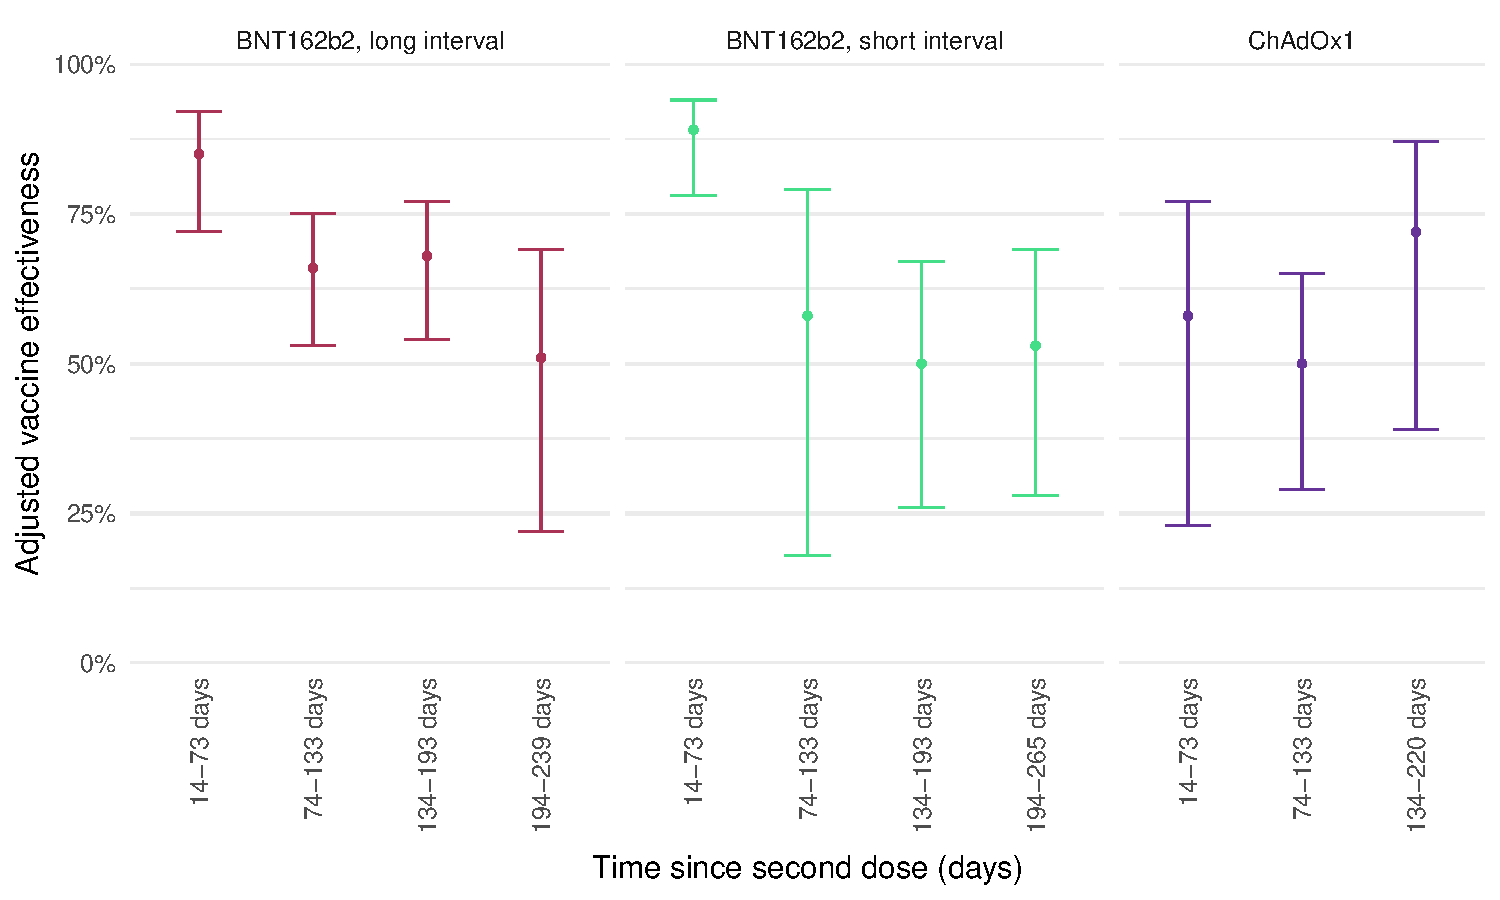
\includegraphics[width=\textwidth]{cox_1.pdf}
    \caption[Adjusted vaccine effectiveness among SIREN participants with no prior infection during the Alpha and Delta variant circulating period]{Adjusted vaccine effectiveness among SIREN participants with no prior infection during the Alpha and Delta variant circulating period, by vaccine type and dosing interval.}\label{fig:cox_1}
\end{figure}

\subsection{Vaccine effectiveness against Omicron}

Cox proportional hazards models were next applied to estimate the effectiveness of third BNT162b2 vaccine doses and previous infection against the Omicron BA.1 and BA.2 sub-variants compared to Delta~\parencite{Hall2024-ai}. This analysis included 19,614 participants, with 29\% having been previously infected. Between September 2021 and February 2022, 95\% received a third vaccine dose and there were 2745 primary infections and 966 reinfections detected during the 6-month follow-up period.

Third dose vaccine effectiveness against the Delta variant for participants who had initially received the BNT162b2 vaccine was 63\% (95\% CI 40 to 77\%) within 0-to-2 months post-third dose, compared to 35\% (95\% CI 21 to 47\%) against the Omicron BA.1 and BA.2 sub-variants. Participants who had initially received the ChAdOX1 vaccine had a median vaccine effectiveness $\geq$68\% against both variants (Figure~\ref{fig:cox_2} panel A). Third dose protection waned rapidly against the Omicron variant, however, with only around 4 months of additional protection conferred by vaccination. Previous infection provided longer-lasting protection against Omicron, 67\% (95\% CI 56 to 75\%) at 3--6 months post-infection, this reduced to 27\% (95\% CI 4 to 44\%) after 9 months, approximately three times lower than against Delta (Figure~\ref{fig:cox_2} panel B).

\begin{figure}[htbp!]
    \centering
    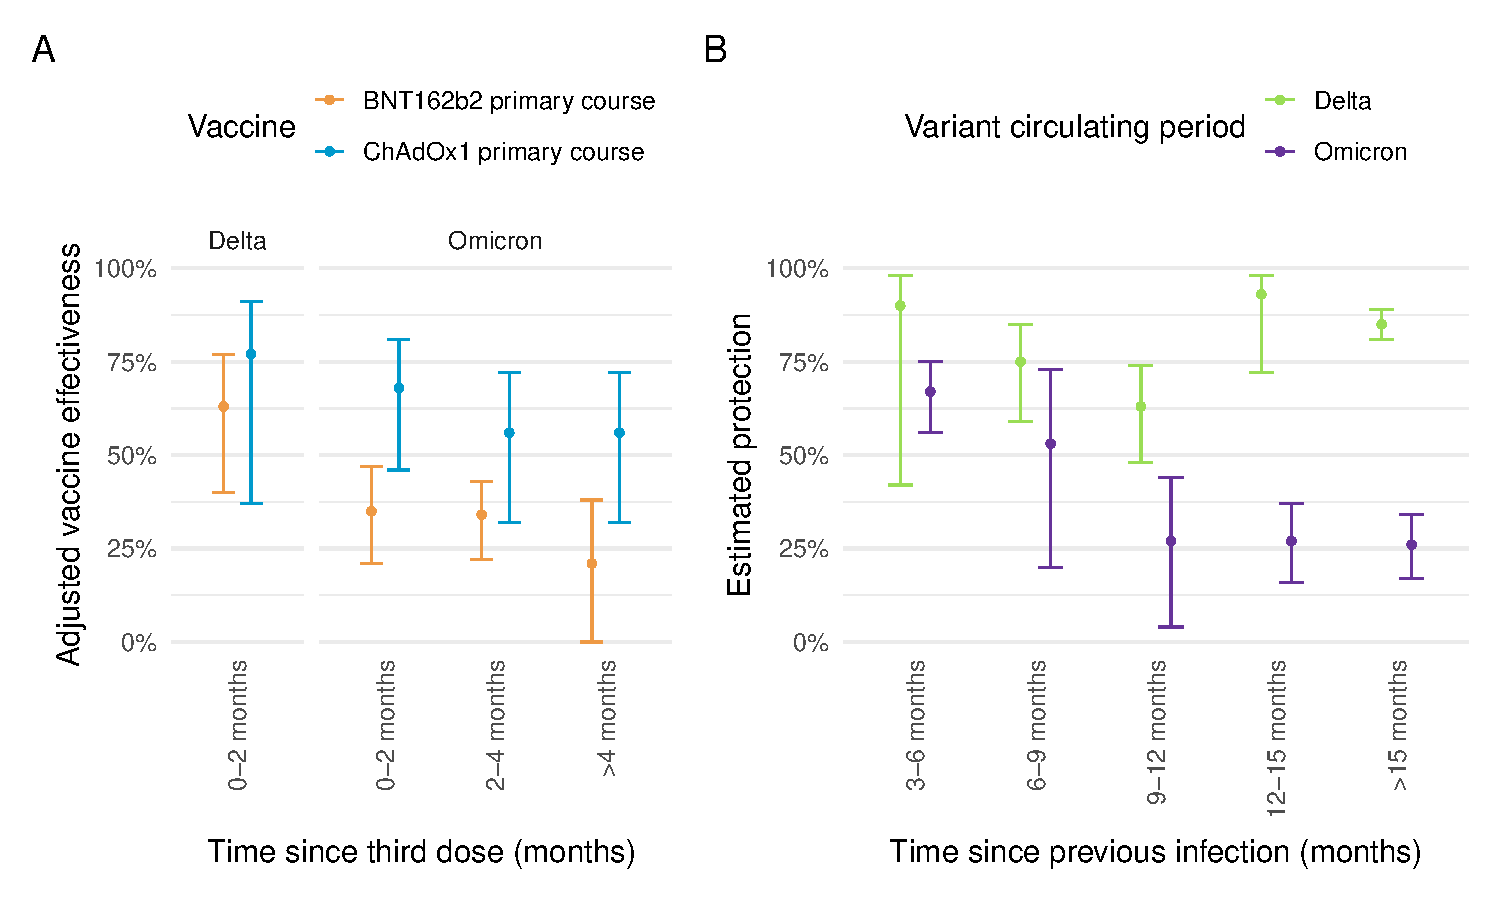
\includegraphics[width=\textwidth]{cox_2.pdf}
    \caption[Third dose vaccine effectiveness and protection against infection, by primary course, time since previous infection, and variant circulating period]{Third dose vaccine effectiveness, by primary course, variant circulating period, and time since vaccination (panel A) and protection against infection, by time since previous infection and variant circulating period (Panel B).}\label{fig:cox_2}
\end{figure}

\subsection{Discussion}

Stratified Cox proportional hazards models were successfully applied to estimate vaccine effectiveness and protection from prior infection in a densely-sampled cohort of healthcare workers with high vaccine coverage.

Two doses of the BNT162b2 vaccine were shown to provide high short-term protection which diminished after six months, whereas protection from two doses of the ChAdOX1 vaccine was substantially lower. Third vaccine doses were found to offer additional short-term protection which again swiftly diminished, particularly against Omicron sub-variants. Meanwhile, infection-acquired immunity (especially when boosted by vaccination) provided longer-lasting protection, although protection was substantially reduced against Omicron as compared to previous variants.

A limitation of the Cox proportional hazards approach under less frequent testing conditions is discussed in Section~\ref{sec:cohort-study-design}, which motivated the development of a multi-state modelling approach.

\section{Fourth dose vaccine uptake and model results}

\begingroup\small

\begin{longtable}[t]{>{\raggedright\arraybackslash}p{6cm}ccc}
\caption{\label{tab:siren_vaccine_uptake}Demographic characteristics of SIREN study participants enrolled between 12 September 2022 and 31 March 2023, by fourth dose vaccine coverage.}\\
\toprule
\multicolumn{2}{c}{ } & \multicolumn{2}{c}{\textbf{Fourth dose vaccine coverage}} \\
\cmidrule(l{3pt}r{3pt}){3-4}
\textbf{Characteristic} & \makecell[c]{\textbf{Overall}\ \ \\N = 9,560} & \makecell[c]{\textbf{Waned third dose}\ \ \\N = 2,887} & \makecell[c]{\textbf{Fourth dose}\ \ \\N = 6,673}\\
\midrule
Gender &  &  & \\
\hspace{1em}Male & 1,524 (15.9\%) & 394 (13.6\%) & 1,130 (16.9\%)\\
\hspace{1em}Female & 8,036 (84.1\%) & 2,493 (86.4\%) & 5,543 (83.1\%)\\
Age group &  &  & \\
\hspace{1em}<25 & 71 (0.7\%) & 33 (1.1\%) & 38 (0.6\%)\\
\hspace{1em}25-34 & 828 (8.7\%) & 319 (11.0\%) & 509 (7.6\%)\\
\hspace{1em}35-44 & 2,096 (21.9\%) & 748 (25.9\%) & 1,348 (20.2\%)\\
\hspace{1em}45-54 & 3,702 (38.7\%) & 1,067 (37.0\%) & 2,635 (39.5\%)\\
\hspace{1em}55-64 & 2,637 (27.6\%) & 662 (22.9\%) & 1,975 (29.6\%)\\
\hspace{1em}65+ & 226 (2.4\%) & 58 (2.0\%) & 168 (2.5\%)\\
Ethnicity &  &  & \\
\hspace{1em}White & 8,611 (90.1\%) & 2,522 (87.4\%) & 6,089 (91.2\%)\\
\hspace{1em}Asian & 543 (5.7\%) & 189 (6.5\%) & 354 (5.3\%)\\
\hspace{1em}Black & 179 (1.9\%) & 91 (3.2\%) & 88 (1.3\%)\\
\hspace{1em}Mixed & 126 (1.3\%) & 43 (1.5\%) & 83 (1.2\%)\\
\hspace{1em}Other & 101 (1.1\%) & 42 (1.5\%) & 59 (0.9\%)\\
Medical condition &  &  & \\
\hspace{1em}No medical conditions & 7,038 (73.6\%) & 2,101 (72.8\%) & 4,937 (74.0\%)\\
\hspace{1em}Immunosuppression & 247 (2.6\%) & 135 (4.7\%) & 112 (1.7\%)\\
\hspace{1em}Chronic respiratory condition & 1,193 (12.5\%) & 324 (11.2\%) & 869 (13.0\%)\\
\hspace{1em}Chronic non-respiratory condition & 1,082 (11.3\%) & 327 (11.3\%) & 755 (11.3\%)\\
Staff type &  &  & \\
\hspace{1em}\makecell[l]{Administrative/Executive (office\\based)} & 1,613 (16.9\%) & 442 (15.3\%) & 1,171 (17.5\%)\\
\hspace{1em}Doctor & 1,155 (12.1\%) & 273 (9.5\%) & 882 (13.2\%)\\
\hspace{1em}Nursing & 3,178 (33.2\%) & 1,030 (35.7\%) & 2,148 (32.2\%)\\
\hspace{1em}Healthcare Assistant & 584 (6.1\%) & 210 (7.3\%) & 374 (5.6\%)\\
\hspace{1em}Midwife & 197 (2.1\%) & 74 (2.6\%) & 123 (1.8\%)\\
\hspace{1em}Healthcare Scientist & 434 (4.5\%) & 136 (4.7\%) & 298 (4.5\%)\\
\hspace{1em}Pharmacist & 268 (2.8\%) & 78 (2.7\%) & 190 (2.8\%)\\
\hspace{1em}\makecell[l]{Physiotherapist/Occupational\\Therapist/SALT} & 404 (4.2\%) & 117 (4.1\%) & 287 (4.3\%)\\
\hspace{1em}\makecell[l]{Student (Medical/\\Nursing/Midwifery/Other)} & 232 (2.4\%) & 56 (1.9\%) & 176 (2.6\%)\\
\hspace{1em}Estates/Porters/Security & 185 (1.9\%) & 66 (2.3\%) & 119 (1.8\%)\\
\hspace{1em}Other (non-patient facing) & 169 (1.8\%) & 40 (1.4\%) & 129 (1.9\%)\\
\hspace{1em}Other (patient facing) & 1,141 (11.9\%) & 365 (12.6\%) & 776 (11.6\%)\\
Occupation setting &  &  & \\
\hspace{1em}\makecell[l]{Ambulance/Emergency\\department/Inpatient wards} & 396 (4.1\%) & 147 (5.1\%) & 249 (3.7\%)\\
\hspace{1em}Intensive care & 1,358 (14.2\%) & 477 (16.5\%) & 881 (13.2\%)\\
\hspace{1em}Maternity/Labour ward & 303 (3.2\%) & 96 (3.3\%) & 207 (3.1\%)\\
\hspace{1em}Office & 829 (8.7\%) & 188 (6.5\%) & 641 (9.6\%)\\
\hspace{1em}Outpatient & 3,841 (40.2\%) & 1,227 (42.5\%) & 2,614 (39.2\%)\\
\hspace{1em}Patient-facing (non-clinical) & 502 (5.3\%) & 148 (5.1\%) & 354 (5.3\%)\\
\hspace{1em}Theatres & 87 (0.9\%) & 27 (0.9\%) & 60 (0.9\%)\\
\hspace{1em}Other & 2,244 (23.5\%) & 577 (20.0\%) & 1,667 (25.0\%)\\
Patient contact &  &  & \\
\hspace{1em}Yes & 7,992 (83.6\%) & 2,466 (85.4\%) & 5,526 (82.8\%)\\
\hspace{1em}No & 1,568 (16.4\%) & 421 (14.6\%) & 1,147 (17.2\%)\\
Index of multiple deprivation &  &  & \\
\hspace{1em}Most deprived (1) & 823 (9.1\%) & 292 (10.7\%) & 531 (8.4\%)\\
\hspace{1em}Deprivation 2 & 1,528 (16.9\%) & 507 (18.6\%) & 1,021 (16.2\%)\\
\hspace{1em}Deprivation 3 & 1,962 (21.7\%) & 574 (21.0\%) & 1,388 (22.0\%)\\
\hspace{1em}Deprivation 4 & 2,121 (23.5\%) & 604 (22.1\%) & 1,517 (24.1\%)\\
\hspace{1em}Least deprived (5) & 2,593 (28.7\%) & 754 (27.6\%) & 1,839 (29.2\%)\\
\hspace{1em}Unknown & 533 & 156 & 377\\
Region &  &  & \\
\hspace{1em}East Midlands & 517 (5.4\%) & 110 (3.8\%) & 407 (6.1\%)\\
\hspace{1em}East of England & 1,176 (12.3\%) & 270 (9.4\%) & 906 (13.6\%)\\
\hspace{1em}London & 1,199 (12.5\%) & 394 (13.6\%) & 805 (12.1\%)\\
\hspace{1em}North East & 223 (2.3\%) & 60 (2.1\%) & 163 (2.4\%)\\
\hspace{1em}North West & 794 (8.3\%) & 212 (7.3\%) & 582 (8.7\%)\\
\hspace{1em}Northern Ireland & 499 (5.2\%) & 133 (4.6\%) & 366 (5.5\%)\\
\hspace{1em}Scotland & 1,701 (17.8\%) & 919 (31.8\%) & 782 (11.7\%)\\
\hspace{1em}South East & 947 (9.9\%) & 210 (7.3\%) & 737 (11.0\%)\\
\hspace{1em}South West & 958 (10.0\%) & 193 (6.7\%) & 765 (11.5\%)\\
\hspace{1em}Wales & 230 (2.4\%) & 38 (1.3\%) & 192 (2.9\%)\\
\hspace{1em}West Midlands & 700 (7.3\%) & 239 (8.3\%) & 461 (6.9\%)\\
\hspace{1em}Yorkshire and the Humber & 616 (6.4\%) & 109 (3.8\%) & 507 (7.6\%)\\
Household structure &  &  & \\
\hspace{1em}\makecell[l]{Lives with others\\(including children)} & 3,570 (37.3\%) & 1,192 (41.3\%) & 2,378 (35.6\%)\\
\hspace{1em}Lives with others (no children) & 4,834 (50.6\%) & 1,383 (47.9\%) & 3,451 (51.7\%)\\
\hspace{1em}Lives alone & 1,156 (12.1\%) & 312 (10.8\%) & 844 (12.6\%)\\
\bottomrule
\end{longtable}

\endgroup

\begin{table}[!h]
\centering\centering
\caption{\label{tab:pcr_positivity}Crude PCR positivity rates per 10,000 person-days and estimated vaccine effectiveness and protection from prior infection by vaccination status, time since previous infection and reported COVID symptoms.}
\centering
\resizebox{\ifdim\width>\linewidth\linewidth\else\width\fi}{!}{
\begin{threeparttable}
\begin{tabular}[t]{l>{\raggedleft\arraybackslash}p{1.5cm}>{\raggedleft\arraybackslash}p{1cm}>{\raggedleft\arraybackslash}p{1.7cm}>{\raggedright\arraybackslash}p{2.3cm}>{\raggedright\arraybackslash}p{1.9cm}>{\raggedleft\arraybackslash}p{1cm}>{\raggedright\arraybackslash}p{1.9cm}>{\raggedleft\arraybackslash}p{1cm}>{\raggedright\arraybackslash}p{1.9cm}}
\toprule
\multicolumn{6}{c}{ } & \multicolumn{2}{c}{Symptomatic} & \multicolumn{2}{c}{Asymptomatic} \\
\cmidrule(l{3pt}r{3pt}){7-8} \cmidrule(l{3pt}r{3pt}){9-10}
\multicolumn{1}{l}{ } & \multicolumn{1}{>{\raggedright\arraybackslash}p{1.5cm}}{Number of participants} & \multicolumn{1}{>{\raggedright\arraybackslash}p{1cm}}{Positive PCR tests} & \multicolumn{1}{>{\raggedright\arraybackslash}p{1.7cm}}{Exposure (person-days at risk)} & \multicolumn{1}{>{\raggedright\arraybackslash}p{2.3cm}}{Crude PCR positivity rate per 10,000 person-days (95\% CI)} & \multicolumn{1}{>{\raggedright\arraybackslash}p{1.9cm}}{Protection relative to baseline (95\% CI)} & \multicolumn{1}{>{\raggedright\arraybackslash}p{1cm}}{Positive PCR tests} & \multicolumn{1}{>{\raggedright\arraybackslash}p{1.9cm}}{Protection relative to baseline (95\% CI)} & \multicolumn{1}{>{\raggedright\arraybackslash}p{1cm}}{Positive PCR tests} & \multicolumn{1}{>{\raggedright\arraybackslash}p{1.9cm}}{Protection relative to baseline (95\% CI)}\\
\midrule
Whole population & 9560 & 1298 & 1521928 & 8.53 (8.07, 9.01) & N/A & 865 & N/A & 265 & N/A\\
\addlinespace[0.3em]
\multicolumn{10}{l}{Vaccination status}\\
\hspace{1em}\makecell[l]{Waned third\\dose} & 9389 & 541 & 603023 & 8.97 (8.23, 9.76) & Baseline & 340 & Baseline & 118 & Baseline\\
\hspace{1em}Fourth dose & 6345 & 757 & 918905 & 8.24 (7.66, 8.85) & 13.08\% (0.89, 23.76) & 525 & 8.55\% (-5.75, 20.91) & 147 & 27.99\% (6.61, 44.48)\\
\addlinespace[0.3em]
\multicolumn{10}{l}{Time since fourth dose}\\
\hspace{1em}0-2 months & 6345 & 179 & 338530 & 5.29 (4.54, 6.12) & 23.97\% (8.48, 36.83) & 131 & 18.52\% (0.08, 33.56) & 34 & 39.85\% (11.24, 59.23)\\
\hspace{1em}2-4 months & 5759 & 300 & 305192 & 9.83 (8.75, 11.01) & 10.3\% (-11.4, 27.78) & 212 & 5.8\% (-18.81, 25.31) & 52 & 26.31\% (-8.34, 49.88)\\
\hspace{1em}4-6 months & 5005 & 278 & 275183 & 10.1 (8.95, 11.36) & 1.71\% (-16.97, 17.4) & 182 & -1.95\% (-23.36, 15.74) & 61 & 15.56\% (-18.18, 39.66)\\
\addlinespace[0.3em]
\multicolumn{10}{l}{Time since previous infection}\\
\hspace{1em}\makecell[l]{Confirmed\\naive} & 773 & 173 & 115165 & 15.02 (12.87, 17.43) & 7.71\% (-35.45, 37.11) & 124 & 16.06\% (-29.03, 45.39) & 33 & -18.47\% (-155.83, 45.13)\\
\hspace{1em}2+ years & 1752 & 196 & 222783 & 8.8 (7.61, 10.12) & Baseline & 127 & Baseline & 40 & Baseline\\
\hspace{1em}1-2 years & 2850 & 209 & 195715 & 10.68 (9.28, 12.23) & 18.35\% (-17.15, 43.09) & 136 & 26.49\% (-10.35, 51.04) & 39 & 5.35\% (-101.67, 55.58)\\
\hspace{1em}6-12 months & 4123 & 347 & 426815 & 8.13 (7.3, 9.03) & 29.08\% (3.82, 47.71) & 226 & 33.85\% (7.48, 52.71) & 81 & 10.56\% (-68.56, 52.55)\\
\hspace{1em}0-6 months & 3433 & 83 & 254866 & 3.26 (2.59, 4.04) & 63.58\% (46.85, 75.04) & 38 & 71.99\% (56.11, 82.13) & 30 & 43.23\% (-17.83, 72.65)\\
\bottomrule
\end{tabular}
\begin{tablenotes}
\item \textit{Note: } 
\item Participants joined the analysis at the date of their first PCR test after 12th September 2022. 171 participants had received their fourth dose booster on or before the date of their first PCR test and contributed no follow-up time in the waned third dose vaccine status.
\end{tablenotes}
\end{threeparttable}}
\end{table}


\begin{table}[!h]
\centering\centering
\caption{\label{tab:sojourn_time}Estimated mean sojourn time in PCR positive state, averaged across the study population, and empirical median duration of PCR positivity by vaccination status and time since previous infection.}
\centering
\begin{tabular}[t]{l>{\raggedright\arraybackslash}p{3.8cm}>{\raggedright\arraybackslash}p{3.8cm}}
\toprule
  & Estimated mean sojourn time in PCR positive state (95\% CI) & Empirical median duration of PCR positivity (initial PCR positive to subsequent PCR negative) [interquartile range]\\
\midrule
Whole population & 7.51 days (6.94, 8.13) & 15 days [12, 27]\\
\addlinespace[0.3em]
\multicolumn{3}{l}{Vaccination status}\\
\hspace{1em}Waned third dose & 8.5 days (6.79, 10.64) & 15 days [13, 28]\\
\hspace{1em}Fourth dose & 6.9 days (5.87, 8.11) & 14 days [12, 26]\\
\addlinespace[0.3em]
\multicolumn{3}{l}{Time since previous infection}\\
\hspace{1em}Confirmed naive & 9.51 days (7.08, 12.78) & 16 days [13, 28]\\
\hspace{1em}2+ years & 9.16 days (7.16, 11.72) & 14 days [12, 27]\\
\hspace{1em}1-2 years & 7.44 days (5.86, 9.44) & 14 days [12, 21]\\
\hspace{1em}6-12 months & 6.56 days (5.63, 7.63) & 14 days [12, 23]\\
\hspace{1em}0-6 months & 7.25 days (6.32, 8.31) & 16 days [14, 28]\\
\addlinespace[0.3em]
\multicolumn{3}{l}{COVID symptoms}\\
\hspace{1em}COVID symptoms & 8.09 days (7.36, 8.9) & 15 days [13, 27]\\
\hspace{1em}\makecell[l]{Non-COVID symptoms\\or asymptomatic} & 4.7 days (4.04, 5.47) & 14 days [12, 23]\\
\bottomrule
\end{tabular}
\end{table}


\clearpage

\section{Alternative model specifications}\label{appendix:alt-models}

\subsection{Convalescent model}

The studies of the SIREN cohort using Cox proportional hazards methodology described in Section~\ref{appendix:siren-cox-models} applied a 90-day episode length, after which point participants were considered to be at risk for reinfection~\parencite{Hall2022-ep, Hall2024-ai}. To emulate this 90-day episode, participants with a negative PCR can be assigned to a recovery (or convalescence) state for a defined period following a positive PCR result (e.g.\ 90 days post-infection). Figure~\ref{fig:ve_convalescent} panels A and B show the estimates from the two-state (main) model and three-state convalescent model.

\begin{figure}[htbp!]
    \centering
    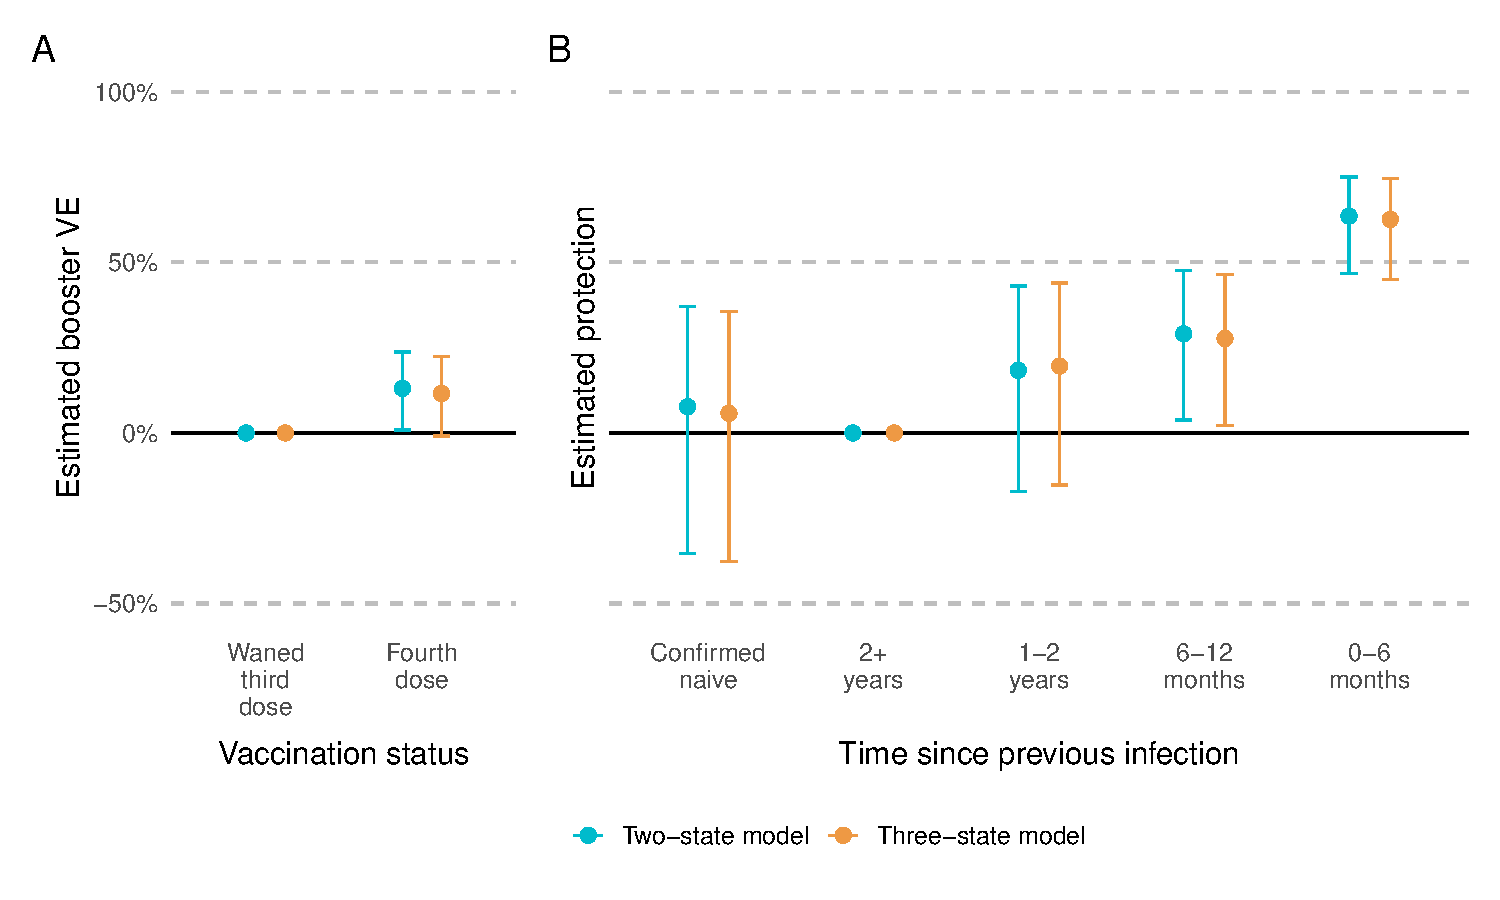
\includegraphics[width=\textwidth]{ve_convalescent.pdf}
    \caption[Estimated booster VE and estimated protection from previous infection in two-state and three-state model]{Estimated booster VE (panel A, model M1) and estimated protection from previous infection (panel B, model M3) in two-state and three-state model. Error bars show the 95\% CI around the estimates.}\label{fig:ve_convalescent}
\end{figure}

\subsection{Semi-Markov model}

Figure~\ref{fig:sojourn_semi_markov} compares mean sojourn times estimated by the Markov model (panel A) to mean sojourn times for long and short stayers estimated by the semi-Markov model (panel B). As expected, the mean sojourn times for the Markov model fall somewhere in between the mean times for the long and short stayers.

\begin{figure}[htbp!]
    \centering
    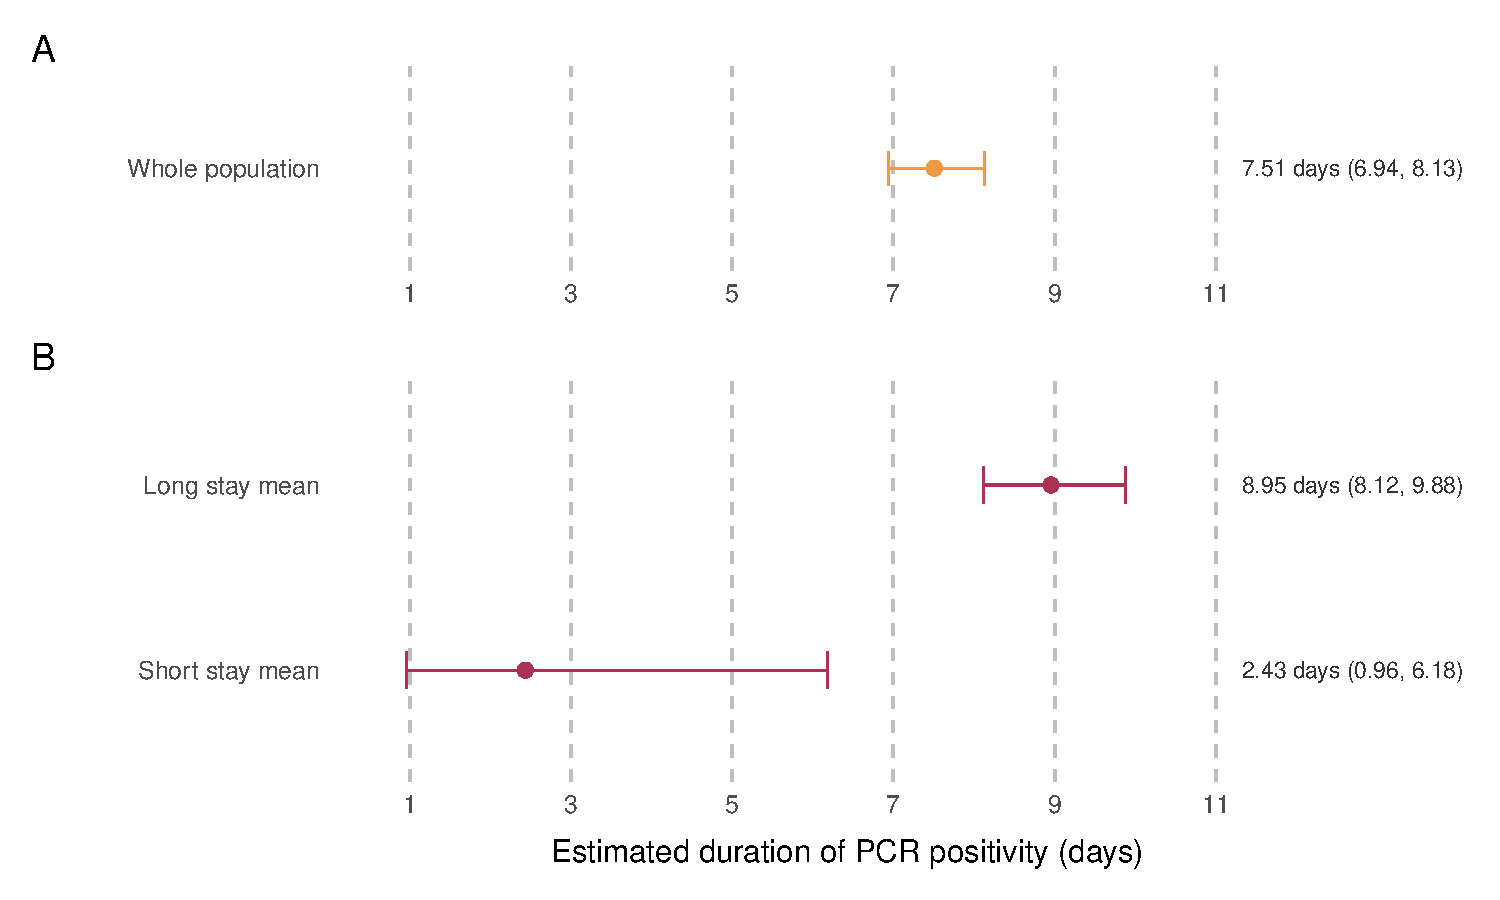
\includegraphics[width=\textwidth]{sojourn_semi_markov.pdf}
    \caption[Estimated mean sojourn time in PCR positive state, averaged across the study population, estimated by Markov and semi-Markov model]{Estimated mean sojourn time in PCR positive state, averaged across the study population, estimated by Markov model (panel A) and semi-Markov model (panel B). Error bars show the 95\% CI around the estimates.}\label{fig:sojourn_semi_markov}
\end{figure}

\subsection{Misclassification model}

Hazards estimated via a misclassification model with fixed misclassification probabilities $\Pr(S \mid P) = 0.09$ and $\Pr(I \mid N) = 0.001$ are shown in Figure~\ref{fig:ve_misclass}. Hazards were similar to those estimated in the two-state model without misclassification, with slightly wider confidence intervals.

\begin{figure}[htbp!]
    \centering
    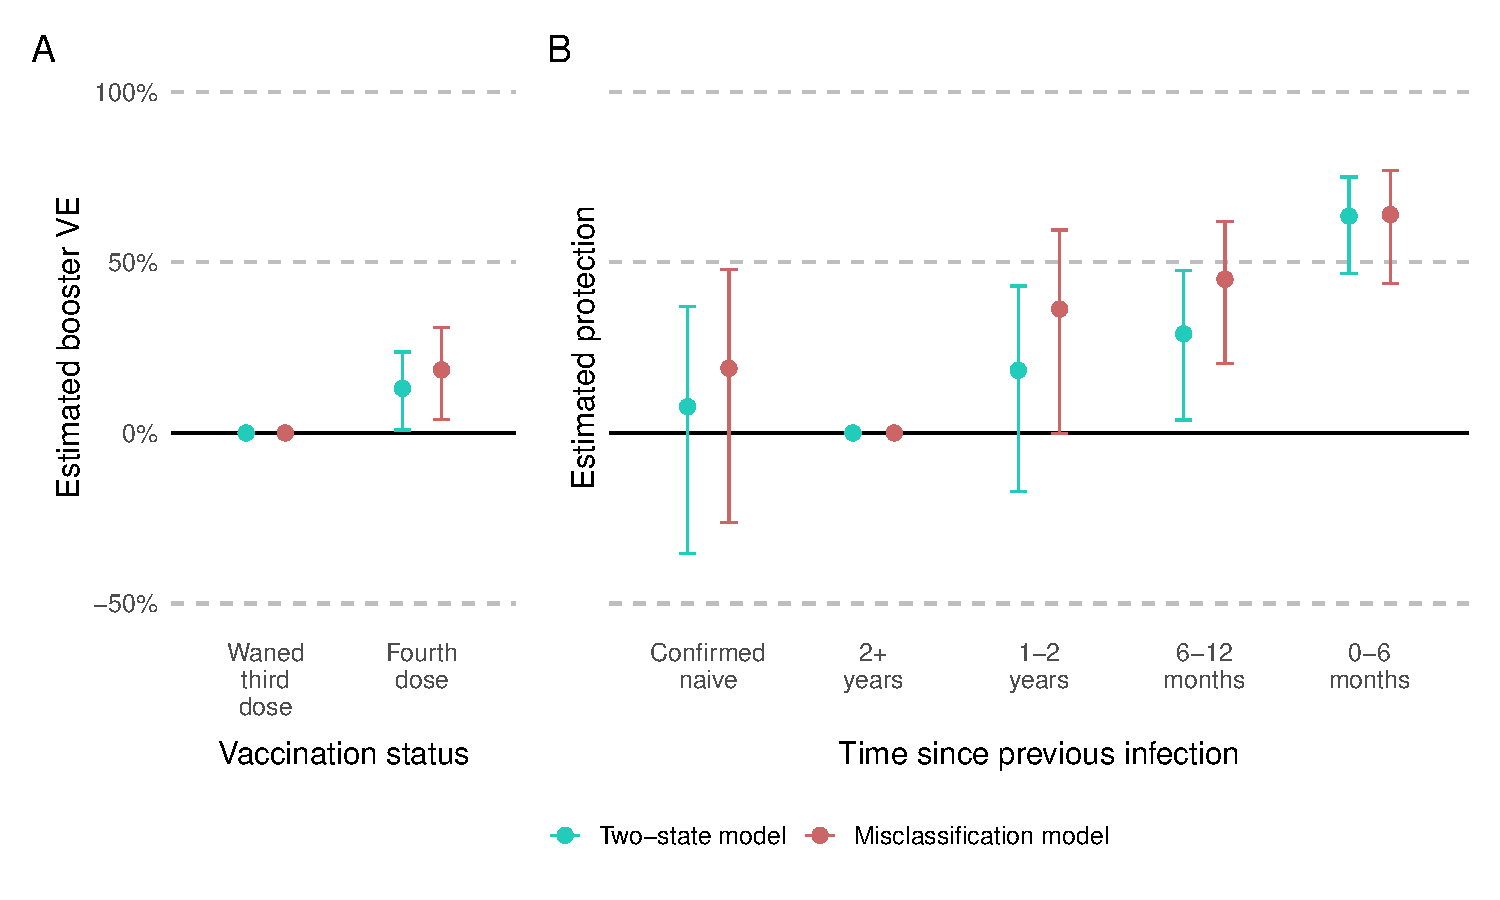
\includegraphics[width=\textwidth]{ve_misclass.pdf}
    \caption[Estimated booster VE and estimated protection from previous infection in two-state and misclassification model]{Estimated booster VE (panel A, model M1) and estimated protection from previous infection (panel B, model M3) in two-state and misclassification model. Error bars show the 95\% CI around the estimates.}\label{fig:ve_misclass}
\end{figure}

\subsection{Na\"{\i}ve baseline model}

`2+ years' was chosen as the baseline category for the time since previous infection covariate in the main analysis. Estimates using the `confirmed na\"{\i}ve' group as the baseline category instead are shown in Figure~\ref{fig:ve_baseline}.

\begin{figure}[htbp!]
    \centering
    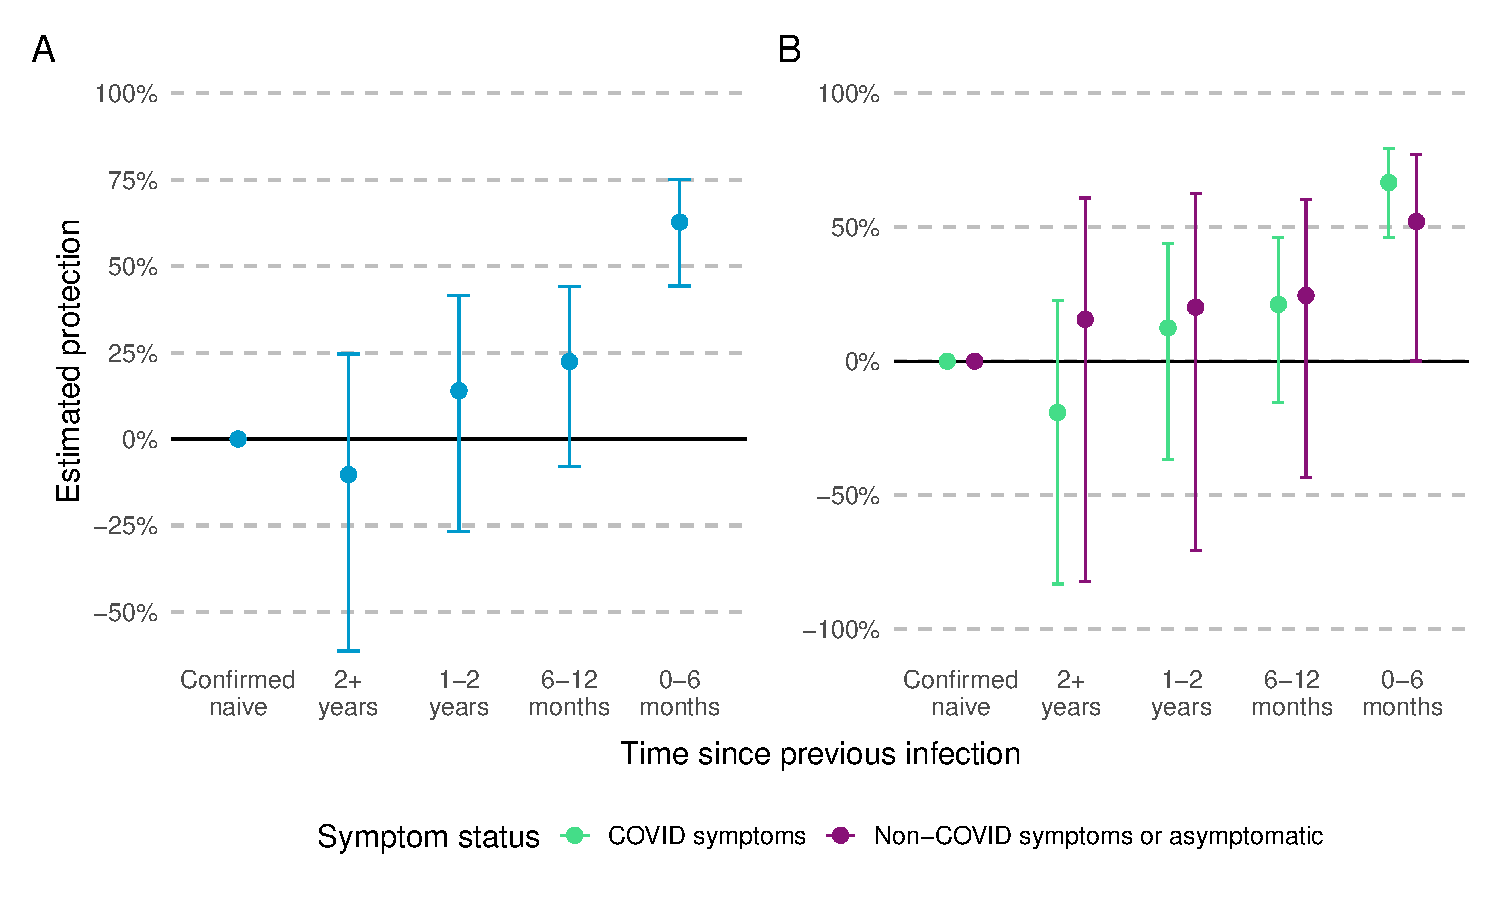
\includegraphics[width=\textwidth]{ve_baseline.pdf}
    \caption[Estimated protection from previous infection relative to confirmed na\"{\i}ve baseline category]{Estimated protection from previous infection, by time since previous infection (panel A, model M3), and symptom status (panel B, model M7), relative to confirmed na\"{\i}ve baseline category. Error bars show the 95\% CI around the estimates.}\label{fig:ve_baseline}
\end{figure}

\section{Cox proportional hazards model comparison}

Figures~\ref{fig:vaccine_long} and ~\ref{fig:vaccine_short_noev} compare hazards estimated by multi-state models M2 and M3 to those from the corresponding stratified Cox proportional hazards model, where the same covariates were included in both models.

\begin{figure}[htbp!]
    \centering
    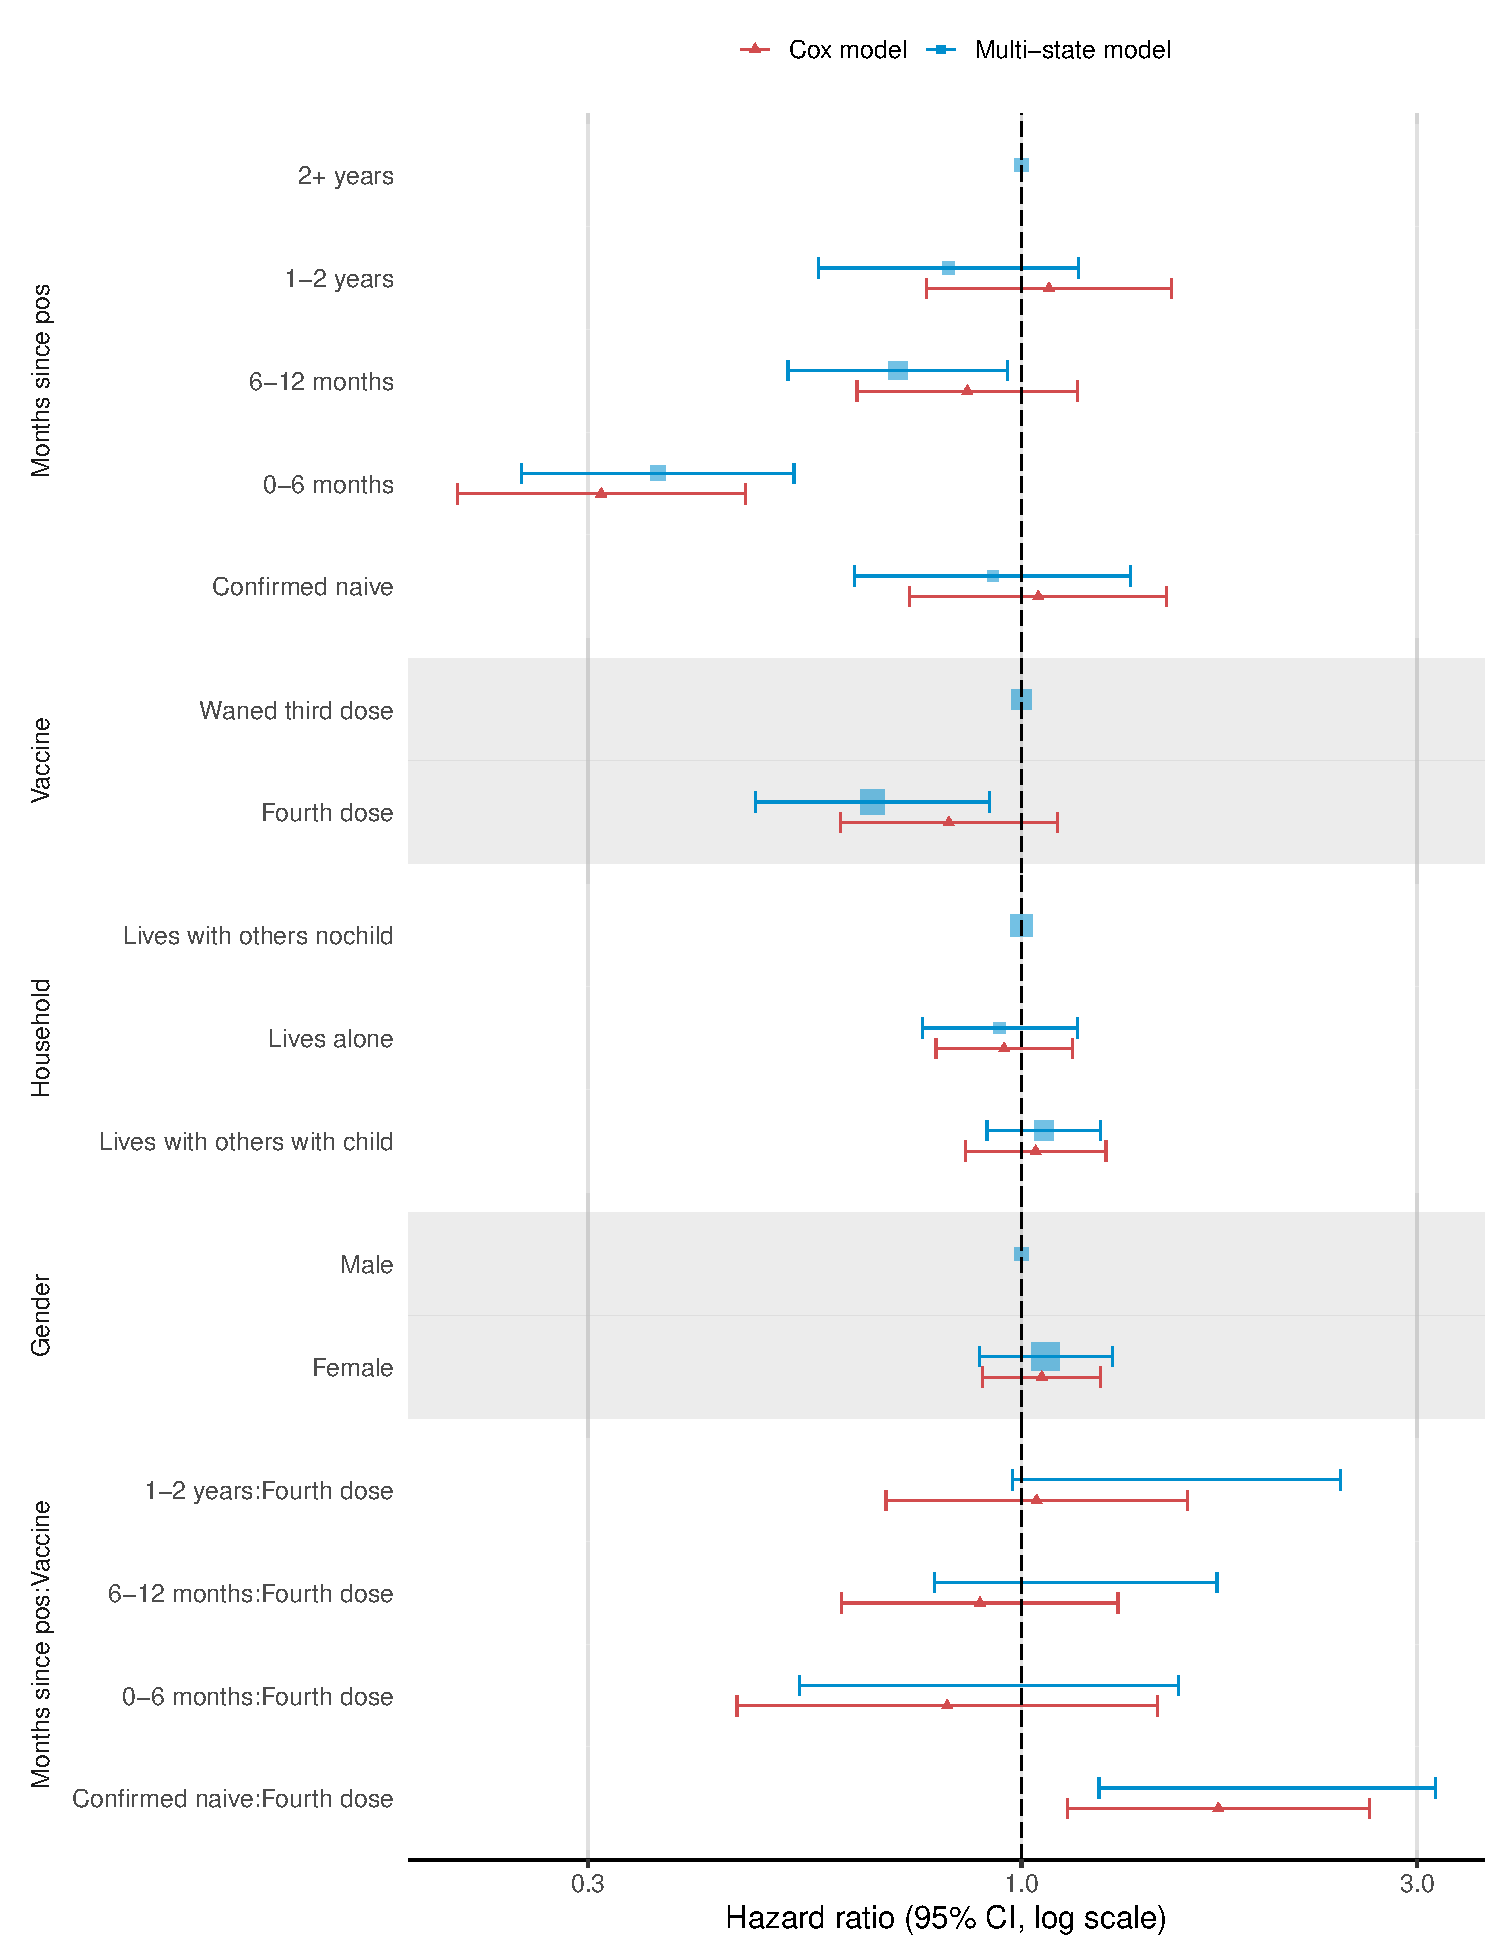
\includegraphics[width=\textwidth]{04_SIREN/Figs/vaccine_short_noev.pdf}
    \caption[Comparison of hazards estimated by multi-state model and the corresponding Cox proportional hazards model]{Comparison of hazards estimated by multi-state model M3 and the corresponding Cox proportional hazards model, for covariates common between the two models. Error bars show the 95\% CI around the estimated hazards.}\label{fig:vaccine_short_noev}
\end{figure}

\begin{figure}[htbp!]
    \centering
    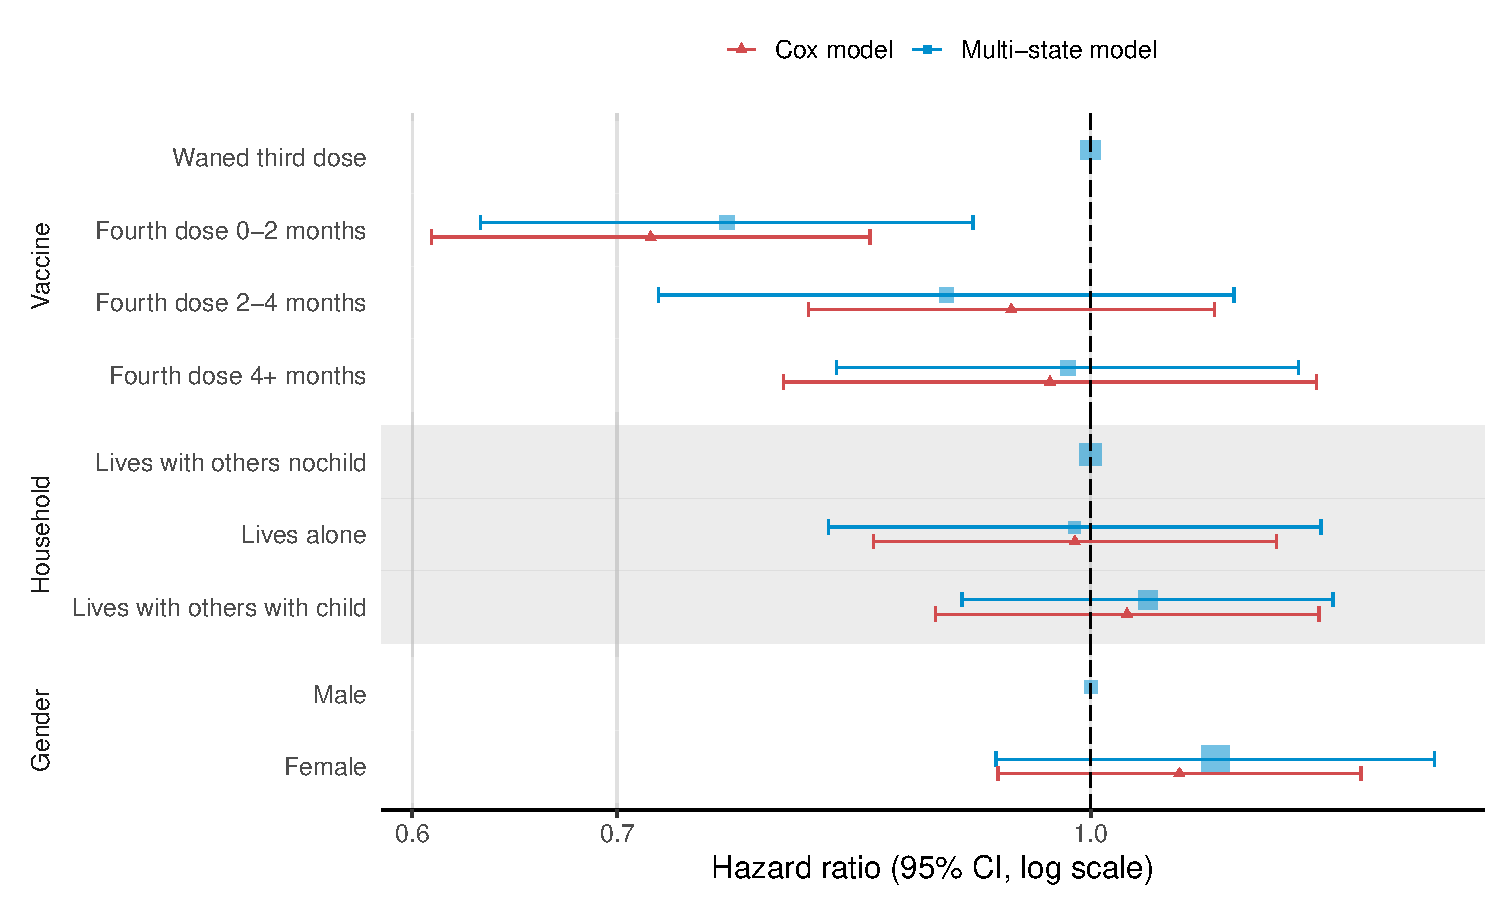
\includegraphics[width=\textwidth]{vaccine_long.pdf}
    \caption[Comparison of hazards estimated by multi-state model and the corresponding Cox proportional hazards model]{Comparison of hazards estimated by multi-state model M2 and the corresponding Cox proportional hazards model, for covariates common between the two models. Error bars show the 95\% CI around the estimated hazards.}\label{fig:vaccine_long}
\end{figure}

\section{Goodness of fit}\label{appendix:siren-gof}

\subsection{Simulated number of infections}
Model M3 was used to simulate the expected number of infections from the fitted model, i.e.\ $\mathbb{E}(N^{I}_{\text{TOT}}; \hat{q}^{I})$, where $N^{I}$ is the counting process for entries into the infected state and $\hat{q}^{I}$ is the maximum likelihood estimate for the transition intensity to the infected state as described in Section~\ref{sec:siren-causal}. 500 simulations were used to infer the variability in this estimate, $\text{Var}(\mathbb{E}(N^{I}_{\text{TOT}}; \hat{q}^{I}))$.

Compared to the observed $n = 1023$ infections, the expected number of infections under the fitted model was 1069 infections (95\% variance 1013 to 1125). With weekly sampling and 100\% adherence to testing, a total of 1310 infections (95\% variance 1242 to 1373) would be expected to have been been detected (Figure~\ref{fig:expected_causal_msm}).

\begin{figure}[htbp!]
    \centering
    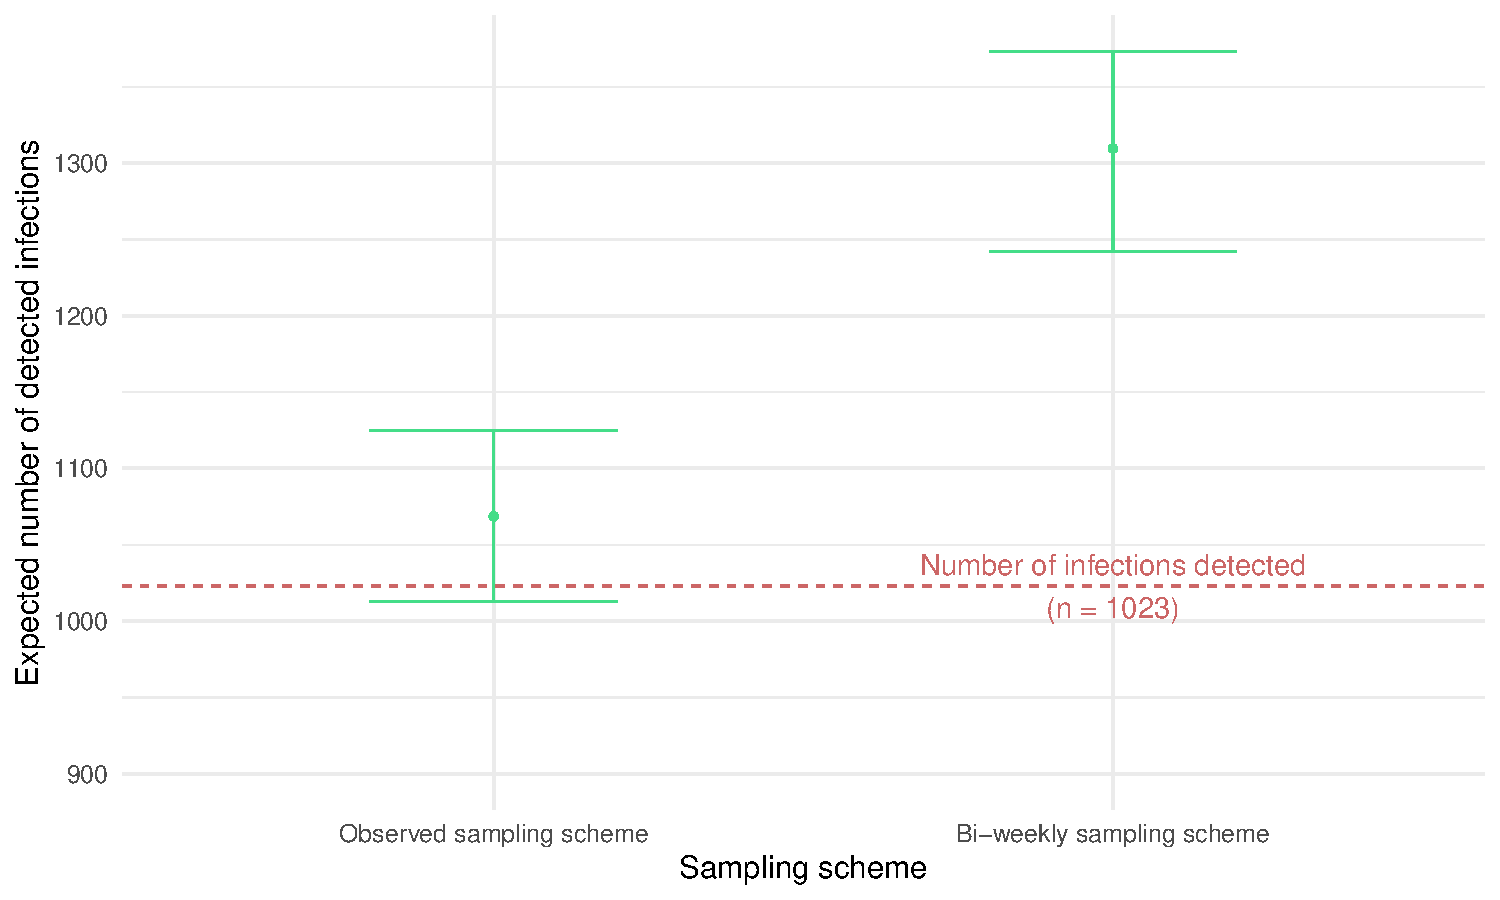
\includegraphics[width=\textwidth]{04_SIREN/Figs/expected_causal_msm.pdf}
    \caption[Expected number of detected infections under observed and bi-weekly sampling schemes]{Expected number of detected infections under observed and bi-weekly sampling schemes with error bars showing variability in the mean estimate, simulated from model M3.}\label{fig:expected_causal_msm}
\end{figure}

\subsection{Causal model goodness of fit}

To assess model fit of the causal model, the number of individuals forecast to be occupying the infected state in the fitted model at a series of times $t$ was compared to an estimate derived from the observed data (Figure~\ref{fig:causal_model_diagnostics}).

\begin{figure}[htbp!]
    \centering
    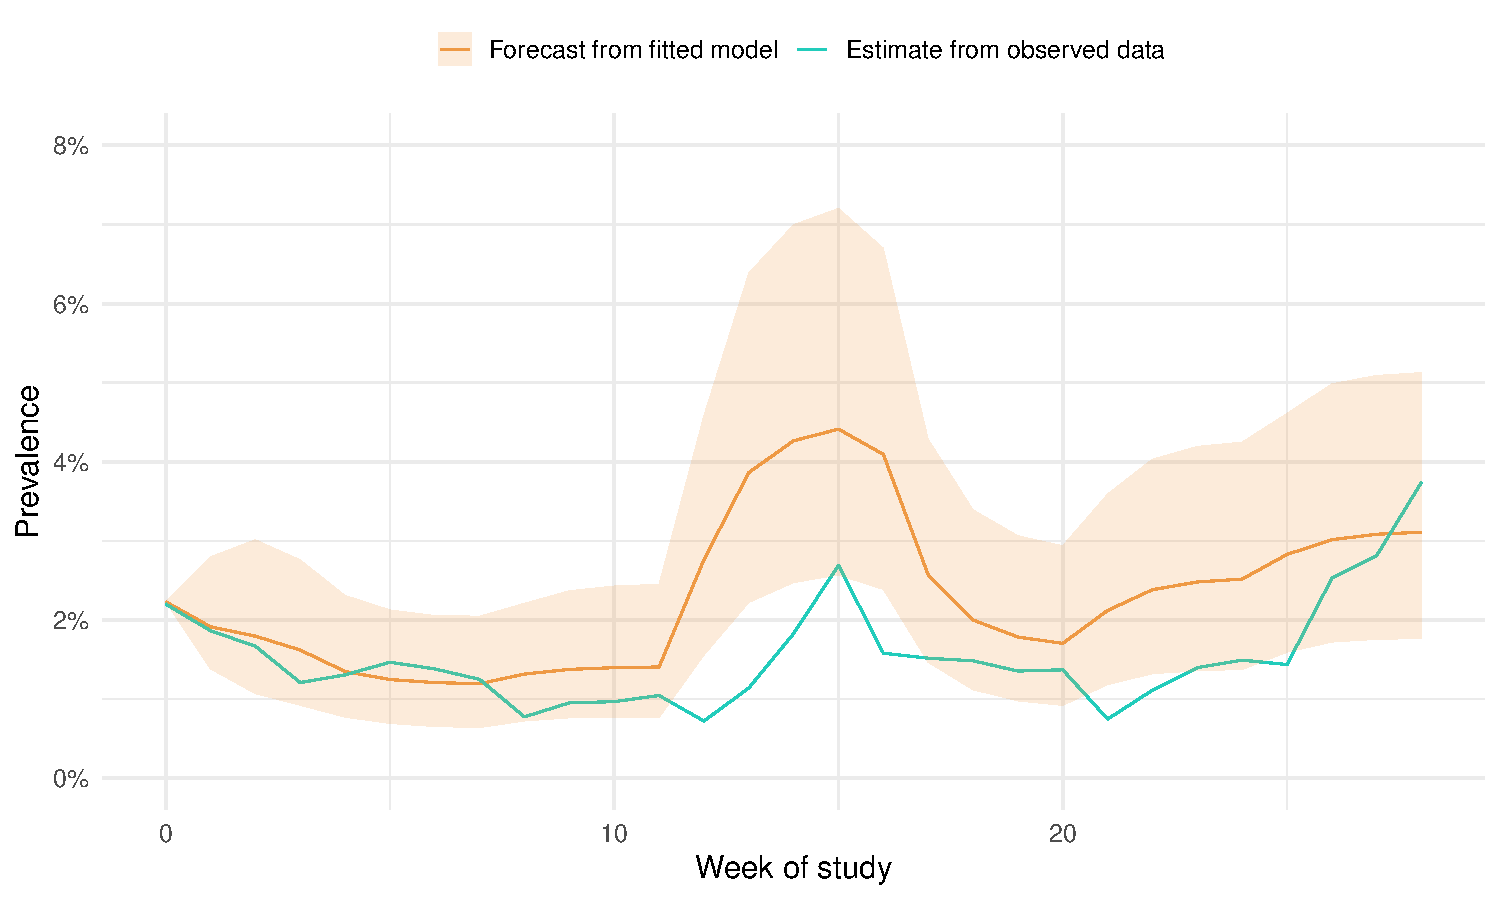
\includegraphics[width=\textwidth]{causal_model_diagnostics.pdf}
    \caption[Comparison of prevalence in the infected state forecast from fitted model and more empirical estimate over time]{Comparison of prevalence in the infected state forecast from fitted model and more empirical estimate over time. Shaded area shows the 95\% CI around the expected prevalence.}\label{fig:causal_model_diagnostics}
\end{figure}